\documentclass{llncs}
\usepackage{graphicx}
\usepackage[braket, qm]{qcircuit}
\usepackage{listings}
\usepackage{amsfonts}
\usepackage{amssymb,amsmath}
\usepackage{pgf,tikz}
\usepackage{comment}
\usepackage{color}
\usetikzlibrary{automata, positioning}
\usetikzlibrary{shapes,arrows}

\newcommand{\C}{\mathbb{C}}
\newcommand{\BC}{B_{\mathbb{C}}}
\newcommand{\half}{\frac{1}{\sqrt{2}}}
\begin{document}

\section{Summary}
Automata theory is widely used to tackle computational problems. Some
quantum versions automata are proposed to study quantum
computation. Real-time quantum automata (QA) are introduced in
\cite{CJ00} by Moore and Crutchfield. Besides, Quantum finite-state
and push-down automata (QFA and QPDA) are defined as special cases of
real-time quantum automata. It is also showed that the corresponding
languages recognized by quantum automata have pleasing properties in
analogy to the classical counterpart. The model by Moore and
Crutchifield is frequently referred as to ``'Measure-Once'
(MO). Another early model is introduced in \cite{AJ97}, which is
referred as to ``Measure-Many'' model (MM).

Early quantum automata models have some limitations, that is to say
they did not embody the full power provided by quantum physics. Their
states are usually vector states in Hilbert spaces, which can only
represent the pure states. Density matrices of self-adjoint positive
mappings of Hilbert spaces with unit trace can represent the mixed
states. The introduction to the Hilbert space formalism of
finite-level quantum systems can be found in \cite{M11}. Moreover, a
general QFA model, which is able to simulate all known QFA, is
proposed in \cite{AA14}.

Coalgebras are widely used to model state-based systems, covering
various flavors of computation, like deterministic, non-deterministic,
probabilistic etc. There are several coalgebraic methods for quantum
computing. A coalgebraic description of quantum walks is proposed in
\cite{B11}, based on the weight functor induced by the complex
numbers. A coalgebraic model of state-based systems that occur in
quantum computation is proposed in \cite{F12}, based on the category
\textbf{Conv} which incorporates both quantum probability via density
matrices and the classical probability that is need for the
output. Although the coalgebraic model can model computations for both
systems in pure states and systems in mixed states, it has some
limitations to model complex quantum systems, like quantum circuits
with measurement and discard. Quantum labeled transition system (QLTS)
based on quantum branching monad in \cite{H14} can cover these
limitations.

\section{Transformation}
Here I try to use the QLTS $(X,s,c)$ in \cite{H14} to model the
coalgebraic model
$$\mathcal{DM}(H)\rightarrow [0,1]^{E}\times \mathcal{DM}(H)^{S}$$ in
\cite{F12}.

Given $dim(H)=n$, $E=\{\epsilon_{1},\dots,\epsilon_{e}\}$ and
$S=\{U_1,\dots,U_s\}$, I define
$X=\{x_0,x_1,\dots,x_s,y_1,\dots,y_e\}$. The pair of functions is
defines as follows:
$$
\begin{aligned}
(s(x_0))_{n,n}&=\lambda \rho\in \mathcal{DM}(H_n). \rho\\
(c(x_i)(x_j))_{n,n}&=\{U_j\}\ \ \ i=0,1,\dots,s\ and\ j=1,\dots,s\\
(c(x_i)(y_j))_{n,n}(\rho)&=\rho \epsilon_{j}\ \ \ \ \ i=0,1,\dots,s\ and\ j=1,\dots,e\\
(c(y_i)(\surd))_{n,n}&=\{I_n\}\ \ \ i=1,\dots,e
\end{aligned}
$$

\begin{example}[\cite{F12}]
  There is a quantum automaton over the alphabet $A=\{a,b\}$. Take the
  two-dimensional state space $\C^{2}$ with the standard basis written
  as $\ket{0}$, $\ket{1}$.The transition matrices are
$$
\delta_a=\half\begin{bmatrix}
1&1 \\
1&-1
\end{bmatrix}, 
\delta_b=\begin{bmatrix}
0&1\\
1&0
\end{bmatrix}.
$$
The initial state is $\varphi_0=\ket{0}$ and the effect is
$\epsilon=\bra{0}\ket{0}$. This automaton can be drawn with the
following state diagram.

\begin{center}
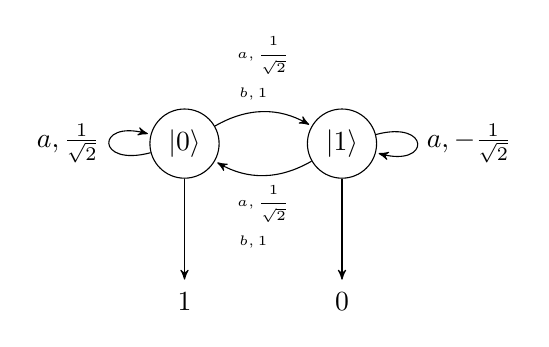
\begin{tikzpicture}[shorten >=1pt,node distance=2cm,on grid,>=stealth']
\node[state] (x_0) {$\ket{0}$};
\node[state] (x_1)  [right=of x_0] {$\ket{1}$};
\node (y_0) [below=of x_0] {1};
\node (y_1) [below=of x_1] {0};
\path[->] (x_0) edge[bend left] node (a_0) [above] {\tiny{$\begin{aligned}a&,\half\\b&,1 \end{aligned}$}}  (x_1)
(x_1) edge[bend left] node [below ] {\tiny{$\begin{aligned}a&,\half\\b&,1 \end{aligned}$}} (x_0)
(x_0) edge (y_0)
(x_1) edge (y_1)
(x_0) edge [loop left] node {$a,\half$} ()
(x_1) edge [loop right] node {$a,-\half$} ();
\end{tikzpicture}
\end{center} 

In \cite{F12}, this quantum automaton $\mathbb{A}=(H,(\delta_a)_{a\in A},\varphi_0,\epsilon)$ gives a coalgebra
$$
\begin{aligned}
\mathcal{DM}(\C^2)&\rightarrow [0,1]\times \mathcal{DM}(\C^2)^{A}\\
\rho&\mapsto(tr(\rho\epsilon),(\delta_a\rho\delta_a^{\dagger})_{a\in A}).
\end{aligned}$$ 

Now this coalgebra gives a QLTS $(X,s,c)$ with the initial state $\bra{0}\ket{0}$, where $X=\{x_0,x_1,x_2,y\}$ and 
$$
\begin{aligned}
(s(x_0))_{2,2}&=\lambda \rho\in \mathcal{DM}(\C^{2}). \rho\\
(c(x_i)(x_j))_{2,2}&=\begin{cases}
\{\delta_a\} &j=1\\
\{\delta_b\} &j=2
\end{cases},\ i=0,1,2\\
(c(x_i)(y))_{2,2}(\rho)&=\rho \epsilon,\ i=0,1,2\\
(c(y)(\surd))_{2,2}&=\{I_2\}.
\end{aligned}
$$


\end{example}

Moreover, if we use a QLTS to model the automaton directly, we can preserve the labels by modifying the pair of functions into follows:
$$
\begin{aligned}
(s(x_0))_{2,2}&=\lambda \rho\in \mathcal{DM}(\C^{2}). \rho\\
(c(x_i)(a,x_1))_{2,2}&=\{\delta_a\},\ i=0,1,2\\
(c(x_i)(b,x_2))_{2,2}&=\{\delta_b\},\ i=0,1,2\\
(c(x_i)(y))_{2,2}(\rho)&=\rho \epsilon,\ i=0,1,2\\
(c(y)(\surd))_{2,2}&=\{I_2\}.
\end{aligned}
$$

\begin{comment}
\begin{theorem}
QLISs in \cite{H14} are more expressive than the coalgebraic models in \cite{F12}.
\end{theorem}

\begin{proof}
To be proved.
\end{proof}
\end{comment}

\section{The monad $\BC$}

%Firstly, we define the category $\mathbf{Sets}$ of sets and partial functions as a suitable working environment for modeling quantum system.

\begin{definition}
The monad $\BC:\mathbf{Sets}\rightarrow \mathbf{Sets}$ is defined as follows:
$$
\begin{aligned}
\BC X&:=\{c:X\rightarrow \C|\sum_{x\in X}c(x)\overline{c(x)}=1\}\\
\BC(f)(c)(y)&:=\begin{cases}0 &f^{-1}(y)=\emptyset\\
\sum_{x\in f^{-1}(y)}c(x) &otherwise
%\BC(f)(c)(y)&:=\begin{cases}0 &f^{-1}(y)=\emptyset\\
%\frac{1}{\sqrt{\alpha}}\sum_{x\in f^{-1}(y)}c(x) &otherwise
\end{cases}
\end{aligned}
$$
%where $$\alpha=\sum_{y\in Y}\sum_{x\in f^{-1}(y)}c(x)\overline{\sum_{x\in f^{-1}(y)}c(x)}.$$

\end{definition}
The unit and the multiplication are:
$$
\begin{aligned}
\eta_{X}(x)&:=\delta_{x}\\
\mu_{X}(\phi)(x)&:=\sum_{c\in B_{\C}(X)}c(x)\phi(c)
\end{aligned}
$$

\begin{definition}
Category $Kl(\BC)$ is defined as follows:
\begin{itemize}
\item $|Kl(\BC)|=|\mathbf{Sets}|$,
\item for any objects $X,Y\in |Kl(B_{\C})|$,
$$Hom_{Kl(B_{\C})}(X,Y)=Hom_{\mathbf{Sets}}(X,\BC Y),$$
\item for any space $X\in |Kl\BC|$, $\eta_X$ is its identity,
\item and, given two $Kl\BC$ arrows $q_1:X\rightarrow \BC Y$, $q_2:Y\rightarrow \BC Z$ their (sequential) composition, denoted by $q_2\bullet q_1$, is equal to $$\mu_Z\cdot \BC q_2\cdot q_1.$$
\end{itemize}
\end{definition}

Given a basis $\ket{x_0},\cdots,\ket{x_{n-1}}$, a state $c_0\ket{x_0}+\cdots+c_{n-1}\ket{x_{n-1}}$ can be modeled as an arrow
$s:1\rightarrow X$ in $Kl(\BC)$, where $s(\ast)({\ket{x_i}})=c_i, i=0,\cdots,n-1$, and a unitary matrix $U$ can be modeled as an arrow $c:X\rightarrow X$ in $kl(\BC)$, where $s(\ket{x_i})(\ket{x_j})=U(i,j).$ Note that it is not required that $\sum_{i=0}^{n-1}c_i\overline{c_i}=1$ here. 

\begin{example}(quantum teleportation protocol)
\[
\Qcircuit @C=.7em @R=.4em @! {
\lstick{\ket{\psi}} & \qw & \qw & \ctrl{1} & \gate{H} & \meter & \control \cw\\
\lstick{\ket{0}} & \qw & \targ & \targ & \qw & \meter & \cwx\\
\lstick{\ket{0}} & \gate{H} & \ctrl{-1} & \qw & \qw & \gate{X} \cwx & \gate{Z} \cwx & \rstick{\ket{\psi}} \qw
}
\]
\end{example}

Given an initial state $\ket{\varphi}=c_0\ket{0}+c_1\ket{1}$, there is a corresponding arrow $s:1\rightarrow X$, where $X=\{\ket{0},\ket{1}\}$ and $s(\ast)(\ket{i})=c_i, i=0,1$. Firstly, we should compose the initial state with $\ket{00}$ by the arrow $c_1:X\rightarrow Y$, where $Y=\{\ket{000},\ket{001},\ket{010},\ket{011},\ket{100},\ket{101},\ket{110},\ket{111}\}$ and 
$$\begin{aligned}
c(\ket{0})(y)&=\begin{cases} 1 &y=\ket{000}\\ 0 &otherwise\end{cases}\\
c(\ket{1})(y)&=\begin{cases} 1 &y=\ket{100}\\ 0 &otherwise\end{cases}.
\end{aligned}
$$. 
The composition of $c_1$ and $s$ is an arrow $c_1\bullet s:1\rightarrow Y$, where 
$$
c_1\bullet s(\ast)(y)=\begin{cases} c_0 & y=\ket{000} \\ c_1 & y=\ket{100} otherwise \end{cases}.
$$
The state transformation corresponds to the arrow $c_2:Y\rightarrow Y$ induced by the unitary operator $(H\otimes I_4)(^cNOT\otimes I_2)(I_2\otimes \ _cNOT)(I_4\otimes H)$, where 
$$
^cNOT=\begin{bmatrix}
1 & 0 & 0 & 0 \\
0 & 1 & 0 & 0 \\
0 & 0 & 0 & 1 \\
0 & 0 & 1 & 0
\end{bmatrix}  
\ _cNOT=\begin{bmatrix}
0 & 1 & 0 & 0 \\
1 & 0 & 0 & 1 \\
0 & 0 & 1 & 0 \\
0 & 1 & 0 & 0
\end{bmatrix}.  
$$
After measuring the top two qubits, there may be four results, corresponding four arrows $m_1,m_2,m_3,m_4:Y\rightarrow X$, where 
$$
\begin{aligned}
m_1(x)(y)&=\begin{cases}1 &x=\ket{000} y=\ket{0}\\ 1 &x=\ket{001} y=\ket{1}\\ 0 & otherwise\end{cases}\\
m_2(x)(y)&=\begin{cases}1 &x=\ket{010} y=\ket{0}\\ 1 &x=\ket{011} y=\ket{1}\\ 0 & otherwise\end{cases}\\
m_3(x)(y)&=\begin{cases}1 &x=\ket{100} y=\ket{0}\\ 1 &x=\ket{101} y=\ket{1}\\ 0 & otherwise\end{cases}\\
m_4(x)(y)&=\begin{cases}1 &x=\ket{110} y=\ket{0}\\ 1 &x=\ket{111} y=\ket{1}\\ 0 & otherwise\end{cases}
\end{aligned}
$$
For different results of the measurement, different operators will be applied to the bottom qubit. Define two arrows $p_x,p_z: X\rightarrow X$ induced by pauli-X matrix and pauli-Z matrix, respectively. There are four corresponding compositions of arrows:
\begin{itemize}
\item if the measurement is $\ket{00}$, the composition is $c_2\bullet c_1\bullet s$;
\item if the measurement is $\ket{01}$, the composition is $p_x\bullet c_2\bullet c_1\bullet s$;
\item if the measurement is $\ket{10}$, the composition is $p_z\bullet c_2\bullet c_1\bullet s$;
\item if the measurement is $\ket{11}$, the composition is $p_z\bullet p_x\bullet c_2\bullet c_1\bullet s$.
\end{itemize}
These composition will get the same arrow $f:1\rightarrow X$, where $f(\ast)(\ket{i})=\frac{1}{2}c_i, i=0,1.$ In quantum mechanics, $s$ and $f$ corresponding to the same state, since the probability of it being found in state $\ket{0}$ or $\ket{1}$ is the same. 


\bibliographystyle{abbrv}
\bibliography{the}
\end{document}